\section{Proportional controller}
\label{sec:proportional_controller}

As explained in the previous section, one of the requests associated with this assignment is to implement a simple proportional controller for the \texttt{Turtlebot3} robot.

For this task, we have opted for a simple two-stage proportional controller.
In particular, based on the distance of the robot from the current target waypoint, we apply a control input so that:

\begin{itemize}
    \item If the robot is far from the target waypoint, we force its direction to be aligned with the target position, and we apply a linear velocity proportional to the distance from the target;
    \item Instead, when the robot is close to the target waypoint, we apply a control input that forces the robot to rotate in place, so that it can align its direction with the direction required by the target waypoint.
\end{itemize}

Some control constraints are also applied.
In particular, we limit the maximum linear velocity to $0.2 \text{ [m/s]}$ and the maximum angular velocity to $0.4 \text{ [rad/s]}$.
Moreover, we consider the robot to be close to the target waypoint when the Euclidean distance from the target waypoint is less than $0.05 \text{ [m]}$.



\subsection{Implementation}
\label{subsec:implementation_proportional_controller}

The code for the implementation of the controller is provided in the Listing \ref{lst:proportional_controller_code}.

\begin{lstlisting}[
    style=Matlab-editor,
    caption={Code for the implementation of the proportional controller.},
    label={lst:proportional_controller_code}
]
function [v, w] = controlProportional(pos_x, pos_y, pos_yaw, target_x, target_y, target_yaw)
% This controller align the robot with the target waypoint and guide it to
% reach it. Once within the threshold zone, correct the yaw of the robot.
% It uses simple Proportional controller for both actions.

bound = @(value, limit) max(min(value, limit), -limit);

% Gains
K_v = 1.2;
K_w = 1.5;
max_linear_speed = 0.2;
max_angular_speed = 0.4;

dx = target_x - pos_x;
dy = target_y - pos_y;
dist_to_target = hypot(dx, dy);
angle_to_target = atan2(dy, dx);

% Control logic
if dist_to_target > 0.05
    v = K_v * dist_to_target;
    w = K_w * wrapToPi(angle_to_target - pos_yaw);
else
    v = 0;
    w = K_w * wrapToPi(target_yaw - pos_yaw);
end

v = bound(v, max_linear_speed);
w = bound(w, max_angular_speed);

end
\end{lstlisting}



\subsection{Results}
\label{subsec:results_proportional_controller}

Given the above implementation of the proportional controller, we can now analyze the results obtained during the simulation.

The results of the obtained trajectory are shown in Figure \ref{fig:proportional_controller_trajectory}, where we report the waypoints highlighted in red and the trajectory of the robot drawn in black.

\begin{figure}[H]
    \centering
    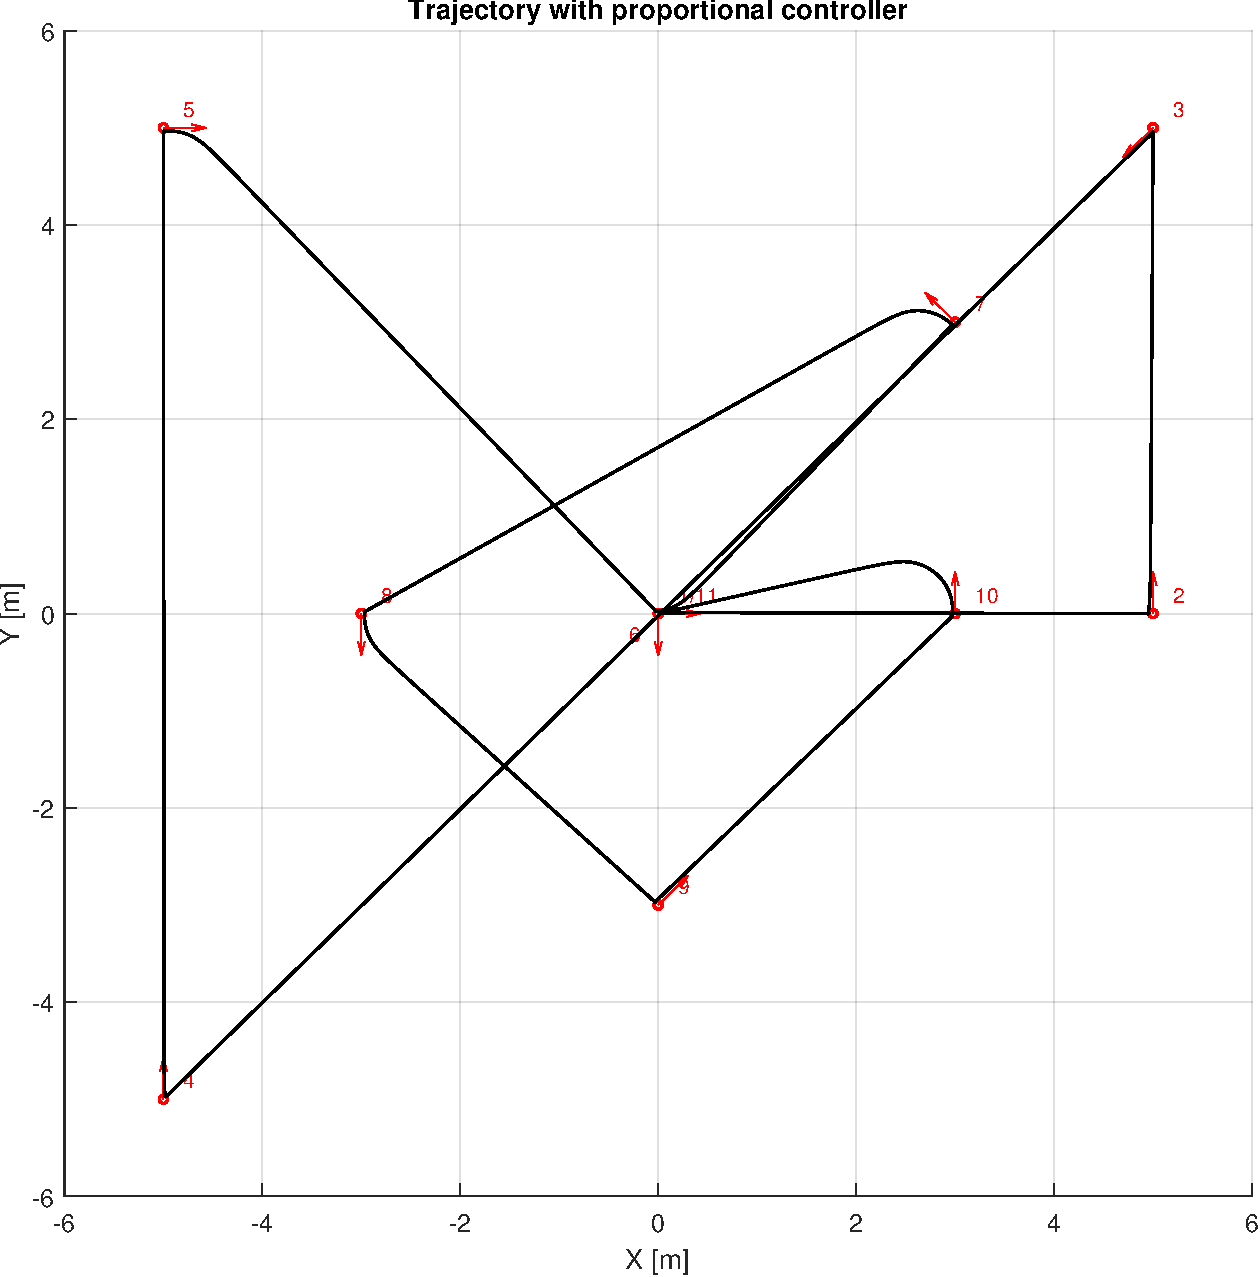
\includegraphics[width=0.6\textwidth]{./img/MATLAB/trajectory_proportional.pdf}
    \caption{Trajectory of the robot during the simulation with the proportional controller.}
    \label{fig:proportional_controller_trajectory}
\end{figure}

One can easily observe that all the waypoints have been reached successfully.

When it comes to the velocity profiles, both in linear and angular dimension, it's easy to visualize the constraints applied to the controller.
The linear velocity is limited to $0.2 \text{ [m/s]}$, while the angular velocity is limited to $0.4 \text{ [rad/s]}$.
This results in a trapezoidal profile for the velocities, as shown in Figure \ref{fig:proportional_controller_velocity_profiles}.

\begin{figure}[H]
    \centering
    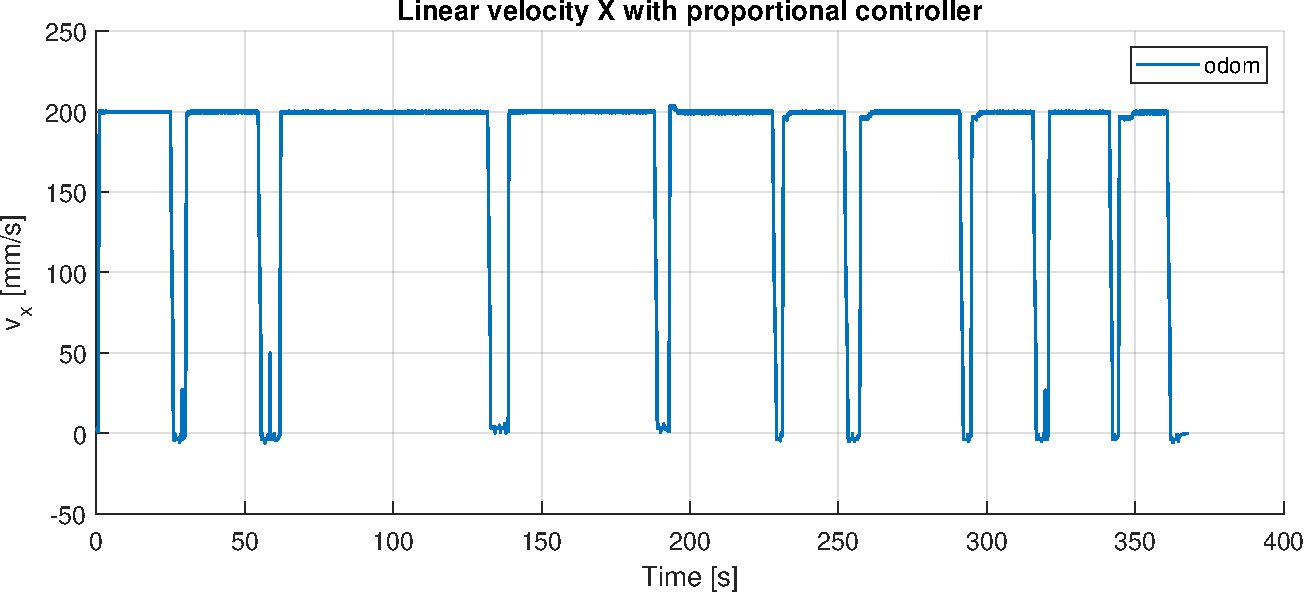
\includegraphics[width=0.7\textwidth]{./img/MATLAB/linear_velocity_proportional.pdf}
    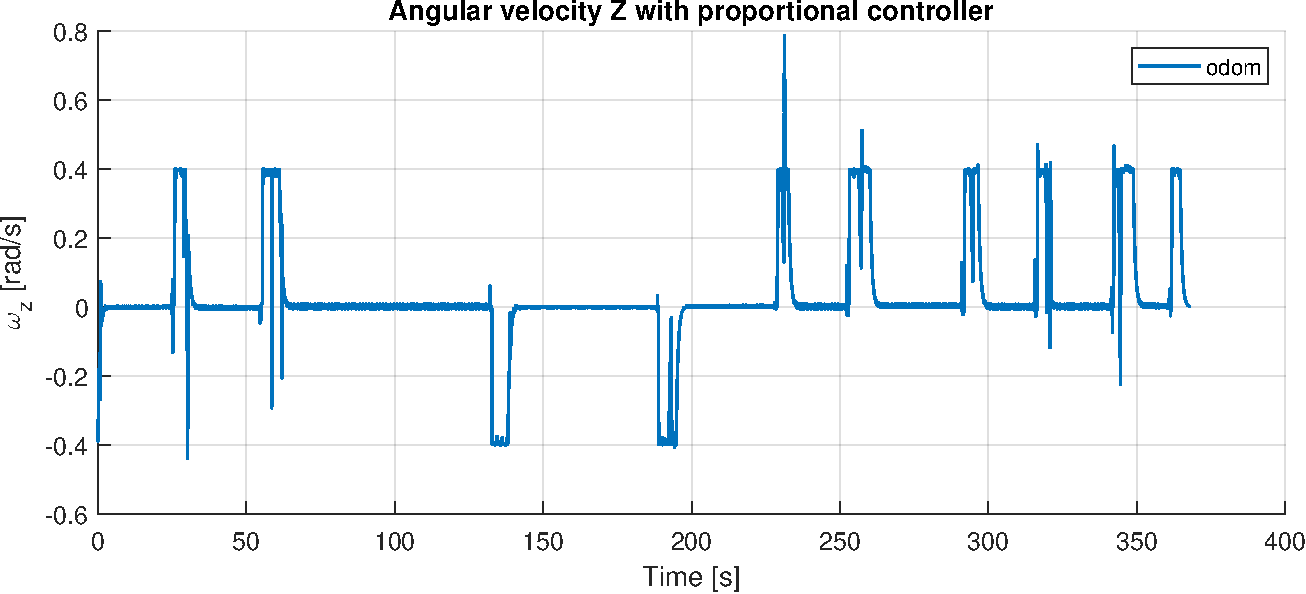
\includegraphics[width=0.7\textwidth]{./img/MATLAB/angular_velocity_proportional.pdf}
    \caption{Velocity profiles of the robot during the simulation with the proportional controller.}
    \label{fig:proportional_controller_velocity_profiles}
\end{figure}

One can also observe some severe (but luckily not too frequent) peaks in the velocities profiles that violate the constraints imposed.
Similarly to the behavior observer in previous assignment, this fact find its explanation in poor performances of the machine on which the simulation is run.
The simulation is run on a virtual machine with limited computational power, which results in some momentary oscillations in the robot's dynamics which are well captured by its telemetries.
We think that a switch to a native environment of \texttt{Ubuntu 20.04} on a \texttt{Linux} kernel machine would solve this issue.
